\ifdefined\inMainDoc\else
\documentclass[12pt,a4paper]{article}
% ================================================================
%  PRÉAMBULE COMMUN - ANNALES CORRIGÉES
%  Université de Kara - FaST - Licence Fondamentale MPC
%  Design optimisé impression noir et blanc
% ================================================================

% -- ENCODAGE & LANGUE --
\usepackage[utf8]{inputenc}
\usepackage[T1]{fontenc}
\usepackage[french]{babel}
\usepackage{lmodern}
\usepackage{microtype}

% -- MISE EN PAGE --
\usepackage[a4paper, top=2.8cm, bottom=2.5cm, left=2.5cm, right=2.5cm, headheight=14pt]{geometry}
\usepackage{setspace}
\setstretch{1.2}
\usepackage{parskip}
\setlength{\parindent}{1.2em}
\setlength{\parskip}{4pt}

% -- MATHS --
\usepackage{amsmath, amssymb, mathtools, amsthm}
\usepackage{mathrsfs}
\usepackage{dsfont}
\usepackage{bm}
\usepackage{cancel}
\usepackage{textcomp}
% Définition de \oiint (intégrale de surface fermée) sans package supplémentaire
\newcommand{\oiint}{\mathop{\iint\!\!\!\!\!\!\!\bigcirc}\limits}

% -- PHYSIQUE & CHIMIE --
\usepackage{physics}
\usepackage{siunitx}
% Lorsque physics est chargé, siunitx omet \qty. On le restaure ici :
\AtBeginDocument{\RenewCommandCopy\qty\SI}
\sisetup{locale = FR, detect-all, output-decimal-marker={,}}
% Commande de substitution pour les unités posant problème avec pdflatex
% (ohm, degreeCelsius, micro, angstrom, percent utilisent des caractères non-ASCII)
\newcommand{\qtyohm}[1]{\ensuremath{\num{#1}\,\Omega}}
\newcommand{\qtydegc}[1]{\ensuremath{\num{#1}\,{}^\circ\text{C}}}
\newcommand{\qtyangstrom}[1]{\ensuremath{\num{#1}\,\text{\AA}}}
\newcommand{\qtypercent}[1]{\ensuremath{\num{#1}\,\%}}
\newcommand{\qtyum}[1]{\ensuremath{\num{#1}\,\mu\text{m}}}
\usepackage[version=4]{mhchem}

% -- GRAPHISMES --
\usepackage{graphicx}
\usepackage{float}
\usepackage{caption}
\usepackage{subcaption}
\usepackage{wrapfig}
\usepackage{tikz}
\usetikzlibrary{calc, arrows.meta, patterns, shapes.geometric}
\usepackage{pgfplots}
\pgfplotsset{compat=1.18}

% -- TABLEAUX --
\usepackage{booktabs}
\usepackage{array}
\usepackage{tabularx}
\usepackage{multirow}

% -- LISTES --
\usepackage{enumitem}
\setlist[enumerate]{topsep=3pt, itemsep=2pt, parsep=0pt}
\setlist[itemize]{topsep=3pt, itemsep=2pt, parsep=0pt, label={.}}

% -- BOÎTES (noir et blanc) --
\usepackage{mdframed}
\usepackage{tcolorbox}
\tcbuselibrary{skins, breakable, theorems}

% Boîte EXERCICE : encadré avec filet épais, fond blanc
\newmdenv[
  linewidth=1.2pt,
  linecolor=black,
  roundcorner=3pt,
  skipabove=10pt,
  skipbelow=6pt,
  innertopmargin=8pt,
  innerbottommargin=8pt,
  innerleftmargin=10pt,
  innerrightmargin=10pt,
  backgroundcolor=white,
  frametitle={\bfseries\small Exercice},
  frametitlealignment=\raggedright,
  frametitleaboveskip=4pt,
  frametitlebelowskip=4pt,
]{boiteexercice}

% Boîte CORRIGÉ : fond gris très clair + filet fin
\newmdenv[
  linewidth=0.6pt,
  linecolor=black,
  leftline=true,
  rightline=false,
  topline=false,
  bottomline=false,
  linecolor=black,
  innerleftmargin=12pt,
  innerrightmargin=8pt,
  innertopmargin=6pt,
  innerbottommargin=6pt,
  backgroundcolor=gray!8,
  skipabove=4pt,
  skipbelow=8pt,
]{boitecorrige}

% Boîte RÉSUMÉ DE COURS : double encadré
\newmdenv[
  linewidth=0.8pt,
  linecolor=black,
  roundcorner=2pt,
  backgroundcolor=gray!12,
  innertopmargin=10pt,
  innerbottommargin=10pt,
  innerleftmargin=12pt,
  innerrightmargin=12pt,
  skipabove=12pt,
  skipbelow=8pt,
]{boiteresume}

% Boîte ATTENTION/REMARQUE : barre gauche épaisse
\newmdenv[
  leftline=true,
  rightline=false,
  topline=false,
  bottomline=false,
  linewidth=3pt,
  linecolor=black,
  backgroundcolor=gray!5,
  innerleftmargin=12pt,
  innerrightmargin=8pt,
  innertopmargin=5pt,
  innerbottommargin=5pt,
  skipabove=6pt,
  skipbelow=6pt,
]{boiteremarque}

% -- DIFFICULTÉ DES EXERCICES --
\newcommand{\facile}{$\star$}
\newcommand{\moyen}{$\star\!\star$}
\newcommand{\difficile}{$\star\!\star\!\star$}
\newcommand{\niveau}[1]{\hfill\textbf{#1}\hspace{2pt}}

% -- EN-TÊTES ET PIEDS DE PAGE --
\usepackage{fancyhdr}
\pagestyle{fancy}
\fancyhf{}
\renewcommand{\headrulewidth}{0.5pt}
\renewcommand{\footrulewidth}{0.3pt}

% -- HYPERLIENS --
\usepackage[hidelinks]{hyperref}
\hypersetup{
    colorlinks=false,
    pdftitle={Annale Corrigée - Licence MPC - Université de Kara}
}

% -- TITRES --
\usepackage{titlesec}
\titleformat{\section}{\Large\bfseries}{\thesection.}{0.8em}{}[\vspace{2pt}\hrule\vspace{4pt}]
\titleformat{\subsection}{\large\bfseries}{\thesubsection.}{0.7em}{}
\titleformat{\subsubsection}{\normalsize\bfseries}{\thesubsubsection.}{0.6em}{}

% -- THÉORÈMES --
\theoremstyle{definition}
\newtheorem{defn}{Définition}[section]
\newtheorem{prop}{Propriété}[section]
\newtheorem{thm}{Théorème}[section]
\newtheorem{corol}{Corollaire}[section]
\newtheorem{exemple}{Exemple}[section]

% -- COMMANDES MATHÉMATIQUES UTILES --
\newcommand{\vect}[1]{\overrightarrow{#1}}
\newcommand{\R}{\mathbb{R}}
\newcommand{\N}{\mathbb{N}}
\newcommand{\Z}{\mathbb{Z}}
\newcommand{\C}{\mathbb{C}}
\renewcommand{\d}{\mathrm{d}}
\newcommand{\deriv}[2]{\dfrac{\d #1}{\d #2}}
\newcommand{\dpart}[2]{\dfrac{\partial #1}{\partial #2}}
\newcommand{\rot}{\overrightarrow{\mathrm{rot}}\,}
\renewcommand{\div}{\mathrm{div}\,}
\renewcommand{\grad}{\overrightarrow{\mathrm{grad}}\,}
\newcommand{\e}{\mathrm{e}}
\newcommand{\ii}{\mathrm{i}}
\renewcommand{\Tr}{\mathrm{Tr}}

% Numérotation des équations par section
\numberwithin{equation}{section}

% -- RÉSULTATS ENCADRÉS --
\newcommand{\res}[1]{\[\boxed{#1}\]}

% -- REMARQUE INLINE --
\newcommand{\rmq}[1]{\begin{boiteremarque}\textbf{Remarque.} #1\end{boiteremarque}}

% -- MISE EN VALEUR DU RÉSULTAT FINAL --
\newcommand{\reponse}[1]{%
  \begin{center}
    \fbox{\begin{minipage}{0.92\textwidth}\centering #1\end{minipage}}
  \end{center}%
}


\lhead{\small\textit{Calcul Intégral - Licence 1}}
\rhead{\small\textit{FaST, Université de Kara}}
\cfoot{\thepage}

\begin{document}
\fi

\begin{center}
  {\LARGE\bfseries CALCUL INTÉGRAL DANS $\mathbb{R}$}\\[0.3cm]
  {\normalsize Licence 1 - Mathématiques, Physique et Chimie}\\[0.1cm]
  \rule{0.7\textwidth}{0.8pt}
\end{center}

\section*{Résumé du cours}

\begin{boiteresume}

\textbf{1. Primitives usuelles.}
\[
\int x^n\,\d x = \frac{x^{n+1}}{n+1}+C \quad (n\neq-1), \quad \int \frac{\d x}{x}=\ln|x|+C, \quad \int\e^x\,\d x=\e^x+C
\]
\[
\int\sin x\,\d x = -\cos x+C, \quad \int\cos x\,\d x=\sin x+C, \quad \int\frac{\d x}{1+x^2}=\arctan x+C
\]
\[
\int\frac{\d x}{\sqrt{1-x^2}}=\arcsin x+C, \quad \int\frac{f'(x)}{f(x)}\,\d x=\ln|f(x)|+C
\]

\textbf{2. Intégration par parties.}
\[
\int u\,\d v = uv - \int v\,\d u, \quad \text{soit} \quad \int u(x)v'(x)\,\d x = [u(x)v(x)] - \int u'(x)v(x)\,\d x.
\]

\textbf{3. Changement de variable.} Si $x=\varphi(t)$ et $\d x=\varphi'(t)\,\d t$ :
$\displaystyle\int f(x)\,\d x = \int f(\varphi(t))\varphi'(t)\,\d t$.

\textbf{4. Décomposition en éléments simples.} Pour une fraction rationnelle $P/Q$ avec $\deg P < \deg Q$, on décompose selon les facteurs de $Q$. Les facteurs linéaires $(x-a)^k$ donnent des termes en $A_i/(x-a)^i$. Les facteurs quadratiques $(x^2+bx+c)^k$ donnent des termes $(Ax+B)/(x^2+bx+c)$.

\textbf{5. Intégrale définie.} $\displaystyle\int_a^b f(x)\,\d x = [F(x)]_a^b = F(b)-F(a)$ où $F$ est une primitive de $f$.

\textbf{6. Intégrales impropres.} $\displaystyle\int_a^{+\infty} f(x)\,\d x = \lim_{M\to+\infty}\int_a^M f(x)\,\d x$ (si la limite existe et est finie, l'intégrale \textit{converge}).

\end{boiteresume}

\newpage
\section{Primitives et techniques d'intégration}

\subsection*{Exercice 1 - Primitives directes \niveau{\facile}}

\begin{boiteexercice}
Calculer les intégrales suivantes :
\begin{enumerate}[label=(\alph*)]
  \item $\displaystyle\int(3x^2 - 2x + 5)\,\d x$
  \item $\displaystyle\int\frac{2x+1}{x^2+x+1}\,\d x$
  \item $\displaystyle\int\frac{\cos x}{\sin^2 x}\,\d x$
  \item $\displaystyle\int x\,\e^{x^2}\,\d x$
  \item $\displaystyle\int\frac{1}{2+3x}\,\d x$
\end{enumerate}
\end{boiteexercice}

\begin{boitecorrige}
\textbf{(a)} $x^3 - x^2 + 5x + C$.

\textbf{(b)} Le numérateur est la dérivée du dénominateur : $\int\frac{f'}{f} = \ln|f|+C$.
$\int\frac{2x+1}{x^2+x+1}\,\d x = \ln(x^2+x+1)+C$ (le dénominateur est toujours positif).

\textbf{(c)} On pose $u=\sin x$, $\d u=\cos x\,\d x$ :
$\int\frac{\cos x}{\sin^2 x}\,\d x = \int\frac{\d u}{u^2} = -\frac{1}{u}+C = -\frac{1}{\sin x}+C$.

\textbf{(d)} On pose $u=x^2$, $\d u=2x\,\d x$ :
$\int x\,\e^{x^2}\,\d x = \frac{1}{2}\int\e^u\,\d u = \frac{\e^{x^2}}{2}+C$.

\textbf{(e)} Forme $\int\frac{\d u}{\alpha u+\beta}=\frac{1}{\alpha}\ln|\alpha u+\beta|+C$ :
$\int\frac{\d x}{2+3x} = \frac{1}{3}\ln|2+3x|+C$.
\end{boitecorrige}

\subsection*{Exercice 2 - Intégration par parties \niveau{\moyen}}

\begin{boiteexercice}
Calculer par parties :
\begin{enumerate}[label=(\alph*)]
  \item $\displaystyle\int x\,\e^x\,\d x$
  \item $\displaystyle\int x\cos x\,\d x$
  \item $\displaystyle\int x^2\ln x\,\d x$
  \item $\displaystyle\int\ln x\,\d x$
  \item $\displaystyle\int\e^x\sin x\,\d x$
\end{enumerate}
\end{boiteexercice}

\begin{boitecorrige}
\textbf{(a)} $u=x$, $\d v=\e^x\d x$ : $\int x\e^x\,\d x = x\e^x - \int\e^x\,\d x = x\e^x - \e^x + C = (x-1)\e^x+C$.

\textbf{(b)} $u=x$, $\d v=\cos x\,\d x$ : $\int x\cos x\,\d x = x\sin x - \int\sin x\,\d x = x\sin x+\cos x+C$.

\textbf{(c)} $u=\ln x$, $\d v=x^2\d x$ : $\int x^2\ln x\,\d x = \frac{x^3}{3}\ln x - \int\frac{x^3}{3}\cdot\frac{1}{x}\,\d x = \frac{x^3}{3}\ln x - \frac{x^3}{9}+C$.

\textbf{(d)} $u=\ln x$, $\d v=\d x$ : $\int\ln x\,\d x = x\ln x - \int\frac{x}{x}\,\d x = x\ln x - x+C$.

\textbf{(e)} Deux intégrations par parties successives. Posons $I=\int\e^x\sin x\,\d x$.

$u=\e^x$, $\d v=\sin x\,\d x$ : $I = -\e^x\cos x + \int\e^x\cos x\,\d x$.

Pour $J=\int\e^x\cos x\,\d x$ : $u=\e^x$, $\d v=\cos x\,\d x$ : $J=\e^x\sin x-\int\e^x\sin x\,\d x = \e^x\sin x-I$.

Donc $I = -\e^x\cos x + \e^x\sin x - I$, soit $2I = \e^x(\sin x-\cos x)$, d'où :
\[
\boxed{I = \frac{\e^x(\sin x - \cos x)}{2}+C}
\]
\end{boitecorrige}

\subsection*{Exercice 3 - Changement de variable \niveau{\moyen}}

\begin{boiteexercice}
Calculer par changement de variable :
\begin{enumerate}[label=(\alph*)]
  \item $\displaystyle\int\frac{x\,\d x}{\sqrt{1-x^2}}$ (poser $u=1-x^2$)
  \item $\displaystyle\int\frac{\d x}{1+\sqrt{x}}$ (poser $u=\sqrt{x}$)
  \item $\displaystyle\int_0^{\pi/2}\sin^3 x\cos x\,\d x$ (poser $u=\sin x$)
  \item $\displaystyle\int_0^1\frac{\d x}{\sqrt{4-x^2}}$ (poser $x=2\sin\theta$)
\end{enumerate}
\end{boiteexercice}

\begin{boitecorrige}
\textbf{(a)} $u=1-x^2$, $\d u=-2x\,\d x$ :
$\int\frac{x\,\d x}{\sqrt{1-x^2}} = -\frac{1}{2}\int\frac{\d u}{\sqrt{u}} = -\frac{1}{2}\cdot2\sqrt{u}+C = -\sqrt{1-x^2}+C$.

\textbf{(b)} $u=\sqrt{x}$, $x=u^2$, $\d x=2u\,\d u$ :
$\int\frac{\d x}{1+\sqrt{x}} = \int\frac{2u\,\d u}{1+u} = 2\int\frac{u\,\d u}{1+u} = 2\int\left(1-\frac{1}{1+u}\right)\d u = 2(u-\ln|1+u|)+C = 2(\sqrt{x}-\ln(1+\sqrt{x}))+C$.

\textbf{(c)} $u=\sin x$, $\d u=\cos x\,\d x$ ; bornes $x=0\Rightarrow u=0$, $x=\pi/2\Rightarrow u=1$ :
$\int_0^{\pi/2}\sin^3 x\cos x\,\d x = \int_0^1 u^3\,\d u = \left[\frac{u^4}{4}\right]_0^1 = \frac{1}{4}$.

\textbf{(d)} $x=2\sin\theta$, $\d x=2\cos\theta\,\d\theta$, $\sqrt{4-x^2}=2\cos\theta$ ; bornes $x=0\Rightarrow\theta=0$, $x=1\Rightarrow\theta=\pi/6$ :
$\int_0^1\frac{\d x}{\sqrt{4-x^2}} = \int_0^{\pi/6}\frac{2\cos\theta\,\d\theta}{2\cos\theta} = \left[\theta\right]_0^{\pi/6} = \frac{\pi}{6}$.
\end{boitecorrige}

\section{Fractions rationnelles et intégrales définies}

\subsection*{Exercice 4 - Décomposition en éléments simples \niveau{\moyen}}

\begin{boiteexercice}
Calculer les intégrales suivantes en décomposant en éléments simples :
\begin{enumerate}[label=(\alph*)]
  \item $\displaystyle\int\frac{\d x}{x^2-1}$
  \item $\displaystyle\int\frac{2x+3}{(x-1)(x+2)}\,\d x$
  \item $\displaystyle\int\frac{x^2}{x^2+1}\,\d x$
\end{enumerate}
\end{boiteexercice}

\begin{boitecorrige}
\textbf{(a)} $\frac{1}{x^2-1}=\frac{1}{(x-1)(x+1)}=\frac{A}{x-1}+\frac{B}{x+1}$.

$A(x+1)+B(x-1)=1$. En $x=1$ : $2A=1\Rightarrow A=\frac{1}{2}$. En $x=-1$ : $-2B=1\Rightarrow B=-\frac{1}{2}$.
\[
\int\frac{\d x}{x^2-1} = \frac{1}{2}\ln|x-1|-\frac{1}{2}\ln|x+1|+C = \frac{1}{2}\ln\left|\frac{x-1}{x+1}\right|+C
\]

\textbf{(b)} $\frac{2x+3}{(x-1)(x+2)}=\frac{A}{x-1}+\frac{B}{x+2}$.

En $x=1$ : $5=3A\Rightarrow A=5/3$. En $x=-2$ : $-1=-3B\Rightarrow B=1/3$.
\[
\int\frac{2x+3}{(x-1)(x+2)}\,\d x = \frac{5}{3}\ln|x-1|+\frac{1}{3}\ln|x+2|+C
\]

\textbf{(c)} Comme $\deg(\text{num})=\deg(\text{den})$, on effectue la division euclidienne : $\frac{x^2}{x^2+1}=1-\frac{1}{x^2+1}$.
\[
\int\frac{x^2}{x^2+1}\,\d x = \int\left(1-\frac{1}{x^2+1}\right)\d x = x-\arctan x+C
\]
\end{boitecorrige}

\subsection*{Exercice 5 - Intégrales définies et aires \niveau{\moyen}}

\begin{boiteexercice}
\begin{enumerate}
  \item Calculer $\displaystyle\int_0^1 x^2\,\e^x\,\d x$.
  \item Calculer l'aire comprise entre les courbes $y=x^2$ et $y=x$ pour $x\in[0,1]$.
  \item Calculer la longueur de l'arc de la parabole $y=x^2$ entre $x=0$ et $x=1$ : $L=\int_0^1\sqrt{1+(y')^2}\,\d x$.
\end{enumerate}
\end{boiteexercice}

\begin{boitecorrige}
\textbf{1.} Deux intégrations par parties successives :
\[
I = [x^2\e^x]_0^1 - 2\int_0^1 x\e^x\,\d x = \e - 2\left([x\e^x]_0^1-\int_0^1\e^x\,\d x\right)
\]
\[
= \e-2\left(\e-(\e-1)\right) = \e-2(1) = \e-2.
\]
\[
\int_0^1 x^2\e^x\,\d x = \e-2 \approx 0{,}718
\]

\textbf{2.} Sur $[0,1]$, $y=x\geq x^2$. Aire :
$\mathcal{A} = \int_0^1(x-x^2)\,\d x = \left[\frac{x^2}{2}-\frac{x^3}{3}\right]_0^1 = \frac{1}{2}-\frac{1}{3} = \frac{1}{6}$.

\textbf{3.} $y'=2x$, donc $(y')^2=4x^2$ :
$L = \int_0^1\sqrt{1+4x^2}\,\d x$.

Changement $x=\frac{1}{2}\sinh t$, $\d x=\frac{1}{2}\cosh t\,\d t$, $\sqrt{1+4x^2}=\cosh t$. Ou par la formule directe :
\[
L = \left[\frac{x\sqrt{1+4x^2}}{2}+\frac{\ln(2x+\sqrt{1+4x^2})}{4}\right]_0^1 = \frac{\sqrt{5}}{2}+\frac{\ln(2+\sqrt{5})}{4} \approx 1{,}479
\]
\end{boitecorrige}

\subsection*{Exercice 6 - Intégrales impropres \niveau{\difficile}}

\begin{boiteexercice}
Étudier la convergence et calculer, si elles convergent :
\begin{enumerate}[label=(\alph*)]
  \item $\displaystyle\int_1^{+\infty}\frac{\d x}{x^2}$
  \item $\displaystyle\int_0^1\frac{\d x}{\sqrt{x}}$
  \item $\displaystyle\int_0^{+\infty}\e^{-x}\,\d x$
  \item $\displaystyle\int_1^{+\infty}\frac{\d x}{x}$ (divergente ?)
\end{enumerate}
\end{boiteexercice}

\begin{boitecorrige}
\textbf{(a)} $\int_1^{+\infty}\frac{\d x}{x^2} = \lim_{M\to+\infty}\left[-\frac{1}{x}\right]_1^M = \lim_{M\to+\infty}\left(-\frac{1}{M}+1\right) = 1$. \textbf{Convergente}, vaut $1$.

\textbf{(b)} Singularité en $x=0$ : $\int_0^1\frac{\d x}{\sqrt{x}} = \lim_{\varepsilon\to0^+}\int_\varepsilon^1 x^{-1/2}\,\d x = \lim_{\varepsilon\to0^+}\left[2\sqrt{x}\right]_\varepsilon^1 = \lim_{\varepsilon\to0^+}(2-2\sqrt{\varepsilon}) = 2$. \textbf{Convergente}, vaut $2$.

\textbf{(c)} $\int_0^{+\infty}\e^{-x}\,\d x = \lim_{M\to+\infty}\left[-\e^{-x}\right]_0^M = \lim_{M\to+\infty}(1-\e^{-M}) = 1$. \textbf{Convergente}, vaut $1$.

\textbf{(d)} $\int_1^{+\infty}\frac{\d x}{x} = \lim_{M\to+\infty}[\ln x]_1^M = \lim_{M\to+\infty}\ln M = +\infty$. \textbf{Divergente}.

En général, $\int_1^{+\infty}\frac{\d x}{x^\alpha}$ converge si et seulement si $\alpha > 1$.
\end{boitecorrige}

\section{Techniques avancées d'intégration}

\subsection*{Exercice 7 - Récurrences et intégrales de Wallis \niveau{\difficile}}

\begin{boiteexercice}
On définit $I_n = \displaystyle\int_0^{\pi/2}\sin^n x\,\d x$ pour $n\geq0$.
\begin{enumerate}
  \item Calculer $I_0$ et $I_1$.
  \item Établir la relation de récurrence $I_n = \dfrac{n-1}{n}\,I_{n-2}$ pour $n\geq2$ par intégration par parties.
  \item En déduire $I_4$, $I_5$ et $I_6$.
  \item Énoncer la formule de Wallis : $\dfrac{\pi}{2} = \dfrac{2\cdot2\cdot4\cdot4\cdot6\cdot6\cdots}{1\cdot3\cdot3\cdot5\cdot5\cdot7\cdots}$.
\end{enumerate}
\end{boiteexercice}

\begin{boitecorrige}
\textbf{1.} $I_0 = \int_0^{\pi/2}1\,\d x = \frac{\pi}{2}$. $I_1 = \int_0^{\pi/2}\sin x\,\d x = [-\cos x]_0^{\pi/2} = 0-(-1) = 1$.

\textbf{2.} On intègre par parties avec $u=\sin^{n-1}x$, $\d v=\sin x\,\d x$ :
\[
I_n = [-\sin^{n-1}x\cos x]_0^{\pi/2} + (n-1)\int_0^{\pi/2}\sin^{n-2}x\cos^2 x\,\d x
\]
Le crochet est nul (sin ou cos s'annulent aux bornes). On remplace $\cos^2 x = 1-\sin^2 x$ :
\[
I_n = (n-1)\int_0^{\pi/2}\sin^{n-2}x(1-\sin^2 x)\,\d x = (n-1)(I_{n-2}-I_n)
\]
\[
I_n + (n-1)I_n = (n-1)I_{n-2} \quad \Rightarrow \quad \boxed{I_n = \frac{n-1}{n}\,I_{n-2}}
\]

\textbf{3.}
$I_4 = \frac{3}{4}I_2 = \frac{3}{4}\cdot\frac{1}{2}I_0 = \frac{3}{4}\cdot\frac{1}{2}\cdot\frac{\pi}{2} = \frac{3\pi}{16}$.

$I_5 = \frac{4}{5}I_3 = \frac{4}{5}\cdot\frac{2}{3}I_1 = \frac{4}{5}\cdot\frac{2}{3} = \frac{8}{15}$.

$I_6 = \frac{5}{6}I_4 = \frac{5}{6}\cdot\frac{3\pi}{16} = \frac{5\pi}{32}$.

\textbf{4.} La formule de Wallis résulte de l'équivalence $I_{2n+1}/I_{2n}\to1$ quand $n\to\infty$, ce qui donne :
\[
\frac{\pi}{2} = \prod_{n=1}^{\infty}\frac{(2n)^2}{(2n-1)(2n+1)} = \frac{2\cdot2\cdot4\cdot4\cdot6\cdot6\cdots}{1\cdot3\cdot3\cdot5\cdot5\cdot7\cdots}
\]
\end{boitecorrige}

\subsection*{Exercice 8 - Fractions rationnelles avancées \niveau{\moyen}}

\begin{boiteexercice}
Calculer les intégrales suivantes :
\begin{enumerate}[label=(\alph*)]
  \item $\displaystyle\int\frac{x^3-1}{x^2-x}\,\d x$
  \item $\displaystyle\int\frac{\d x}{(x-1)^2(x+2)}$
  \item $\displaystyle\int\frac{x+1}{x^2+2x+5}\,\d x$
\end{enumerate}
\end{boiteexercice}

\begin{boitecorrige}
\textbf{(a)} $\deg(\text{num}) > \deg(\text{den})$ : division euclidienne. $x^3-1 = (x^2-x)\cdot x + (x^2-1)$... Procédons autrement : $x^3-1 = (x^2-x)\cdot q(x)+r(x)$.

$x^3\div x^2 = x$, reste $x^3-1-x(x^2-x) = x^2-1$. $x^2-1\div x^2 = 1$, reste $x^2-1-(x^2-x)=x-1$.
\[
\frac{x^3-1}{x^2-x} = x+1+\frac{x-1}{x(x-1)} = x+1+\frac{1}{x}
\]
\[
\int\frac{x^3-1}{x^2-x}\,\d x = \frac{x^2}{2}+x+\ln|x|+C
\]

\textbf{(b)} $\frac{1}{(x-1)^2(x+2)} = \frac{A}{x-1}+\frac{B}{(x-1)^2}+\frac{C}{x+2}$.

En $x=1$ : $B = 1/3$. En $x=-2$ : $C = 1/9$. Coefficient de $x^2$ : $A+C=0$, $A=-1/9$.
\begin{align*}
\int\frac{\d x}{(x-1)^2(x+2)} &= -\frac{1}{9}\ln|x-1|-\frac{1}{3(x-1)}+\frac{1}{9}\ln|x+2|+C\\
&= \frac{1}{9}\ln\left|\frac{x+2}{x-1}\right|-\frac{1}{3(x-1)}+C
\end{align*}

\textbf{(c)} Le numérateur est presque la dérivée de $x^2+2x+5$ qui est $2x+2$. On complète :
$\frac{x+1}{x^2+2x+5} = \frac{1}{2}\cdot\frac{2x+2}{x^2+2x+5}$.
\[
\int\frac{x+1}{x^2+2x+5}\,\d x = \frac{1}{2}\ln(x^2+2x+5)+C
\]
(car $x^2+2x+5 = (x+1)^2+4 > 0$ toujours).
\end{boitecorrige}

\subsection*{Exercice 9 - Calcul de volumes \niveau{\moyen}}

\begin{boiteexercice}
\begin{enumerate}
  \item Calculer le volume du solide de révolution engendré par la rotation autour de l'axe $Ox$ de la courbe $y=\sqrt{x}$ pour $x\in[0,4]$.
  \item Calculer le volume de la boule de rayon $R$ en utilisant la méthode des disques.
  \item Calculer le volume du cône de révolution de rayon de base $r$ et de hauteur $h$.
\end{enumerate}
\end{boiteexercice}

\begin{boitecorrige}
\textbf{1.} Volume de révolution par la méthode des disques :
\[
V = \int_0^4 \pi y^2\,\d x = \pi\int_0^4 x\,\d x = \pi\left[\frac{x^2}{2}\right]_0^4 = \pi\times8 = 8\pi
\]

\textbf{2.} La demi-boule de rayon $R$ est engendrée par $y=\sqrt{R^2-x^2}$, $x\in[-R,R]$ :
\begin{align*}
V &= \pi\int_{-R}^R(R^2-x^2)\,\d x = \pi\left[R^2 x-\frac{x^3}{3}\right]_{-R}^R\\
&= \pi\left[\left(R^3-\frac{R^3}{3}\right)-\left(-R^3+\frac{R^3}{3}\right)\right]
\end{align*}
\[
= \pi\cdot\frac{4R^3}{3} = \frac{4\pi R^3}{3}
\]

\textbf{3.} Pour un cône de rayon $r$ à la base ($x=0$) et de hauteur $h$ (axe $x$), le rayon à la hauteur $x$ est $y(x) = r(1-x/h)$ (section droite linéaire) :
\[
V = \pi\int_0^h r^2\left(1-\frac{x}{h}\right)^2\d x = \pi r^2\int_0^h\left(1-\frac{x}{h}\right)^2\d x
\]
Posons $u = 1-x/h$, $\d u = -\d x/h$ :
\[
V = \pi r^2 h\int_0^1 u^2\,\d u = \pi r^2 h\cdot\frac{1}{3} = \frac{\pi r^2 h}{3}
\]
\end{boitecorrige}

\subsection*{Exercice 10 - Intégrale double \niveau{\difficile}}

\begin{boiteexercice}
Calculer les intégrales doubles suivantes :
\begin{enumerate}[label=(\alph*)]
  \item $\displaystyle\iint_D xy\,\d x\,\d y$ où $D = [0,1]\times[0,2]$.
  \item $\displaystyle\iint_T (x+y)\,\d x\,\d y$ où $T$ est le triangle de sommets $(0,0)$, $(1,0)$, $(0,1)$.
  \item $\displaystyle\iint_D e^{x+y}\,\d x\,\d y$ où $D = [0,1]\times[0,1]$.
\end{enumerate}
\end{boiteexercice}

\begin{boitecorrige}
\textbf{(a)} Par le théorème de Fubini :
\[
\iint_D xy\,\d x\,\d y = \int_0^1 x\,\d x\int_0^2 y\,\d y = \left[\frac{x^2}{2}\right]_0^1\times\left[\frac{y^2}{2}\right]_0^2 = \frac{1}{2}\times2 = 1
\]

\textbf{(b)} Le triangle $T$ est défini par $0\leq x\leq1$, $0\leq y\leq1-x$ :
\[
\iint_T (x+y)\,\d x\,\d y = \int_0^1\d x\int_0^{1-x}(x+y)\,\d y = \int_0^1\left[xy+\frac{y^2}{2}\right]_0^{1-x}\d x
\]
\[
= \int_0^1\left(x(1-x)+\frac{(1-x)^2}{2}\right)\d x = \int_0^1\left(x-x^2+\frac{1-2x+x^2}{2}\right)\d x
\]
\[
= \int_0^1\left(\frac{1}{2}-\frac{x^2}{2}\right)\d x = \left[\frac{x}{2}-\frac{x^3}{6}\right]_0^1 = \frac{1}{2}-\frac{1}{6} = \frac{1}{3}
\]

\textbf{(c)}
\[
\iint_D e^{x+y}\,\d x\,\d y = \int_0^1 e^x\,\d x\int_0^1 e^y\,\d y = (e-1)^2 \approx 2{,}952
\]
\end{boitecorrige}

\subsection*{Exercice 11 - Intégrale de Gauss \niveau{\difficile}}

\begin{boiteexercice}
\begin{enumerate}
  \item Montrer que $I = \displaystyle\int_0^{+\infty}\e^{-x^2}\,\d x = \frac{\sqrt{\pi}}{2}$ en utilisant $I^2 = \int_0^{+\infty}\int_0^{+\infty}\e^{-(x^2+y^2)}\,\d x\,\d y$ et un passage en polaires.
  \item En déduire $\displaystyle\int_{-\infty}^{+\infty}\e^{-x^2}\,\d x = \sqrt{\pi}$.
  \item Calculer $\displaystyle\int_0^{+\infty} x^2\e^{-x^2}\,\d x$.
\end{enumerate}
\end{boiteexercice}

\begin{boitecorrige}
\textbf{1.} $I^2 = \iint_{\text{premier quadrant}}\e^{-(x^2+y^2)}\,\d x\,\d y$.

En coordonnées polaires : $x = r\cos\theta$, $y = r\sin\theta$, $\d x\,\d y = r\,\d r\,\d\theta$, domaine $r\in[0,+\infty[$, $\theta\in[0,\pi/2]$ :
\[
I^2 = \int_0^{\pi/2}\d\theta\int_0^{+\infty}r\e^{-r^2}\,\d r = \frac{\pi}{2}\times\left[-\frac{\e^{-r^2}}{2}\right]_0^{+\infty} = \frac{\pi}{2}\times\frac{1}{2} = \frac{\pi}{4}
\]
Donc $I = \sqrt{\pi}/2$.

\textbf{2.} Par parité de $\e^{-x^2}$ :
\[
\int_{-\infty}^{+\infty}\e^{-x^2}\,\d x = 2I = \sqrt{\pi}
\]

\textbf{3.} Par intégration par parties avec $u = x$, $\d v = x\e^{-x^2}\,\d x$, $v = -\e^{-x^2}/2$ :
\[
\int_0^{+\infty} x^2\e^{-x^2}\,\d x = \left[-\frac{x\e^{-x^2}}{2}\right]_0^{+\infty} + \int_0^{+\infty}\frac{\e^{-x^2}}{2}\,\d x = 0+\frac{1}{2}\cdot\frac{\sqrt{\pi}}{2} = \frac{\sqrt{\pi}}{4}
\]
\end{boitecorrige}

\subsection*{Exercice 12 - Intégrales trigonométriques \niveau{\moyen}}

\begin{boiteexercice}
Calculer les intégrales suivantes :
\begin{enumerate}[label=(\alph*)]
  \item $\displaystyle\int_0^{\pi}\sin^2 x\,\d x$
  \item $\displaystyle\int_0^{\pi/2}\sin^2 x\cos x\,\d x$
  \item $\displaystyle\int\tan^2 x\,\d x$
  \item $\displaystyle\int_0^{\pi/4}\frac{\d x}{\cos^2 x}$
\end{enumerate}
\end{boiteexercice}

\begin{boitecorrige}
\textbf{(a)} En utilisant la formule $\sin^2 x = (1-\cos 2x)/2$ :
\[
\int_0^\pi\sin^2 x\,\d x = \int_0^\pi\frac{1-\cos2x}{2}\,\d x = \left[\frac{x}{2}-\frac{\sin2x}{4}\right]_0^\pi = \frac{\pi}{2}
\]

\textbf{(b)} Posons $u=\sin x$, $\d u=\cos x\,\d x$ ; bornes : $0\to0$, $\pi/2\to1$ :
\[
\int_0^{\pi/2}\sin^2 x\cos x\,\d x = \int_0^1 u^2\,\d u = \frac{1}{3}
\]

\textbf{(c)} $\tan^2 x = \sec^2 x - 1$, donc :
\[
\int\tan^2 x\,\d x = \int(\sec^2 x-1)\,\d x = \tan x - x + C
\]

\textbf{(d)} $1/\cos^2 x = \sec^2 x$ dont la primitive est $\tan x$ :
\[
\int_0^{\pi/4}\frac{\d x}{\cos^2 x} = [\tan x]_0^{\pi/4} = \tan(\pi/4)-\tan(0) = 1-0 = 1
\]
\end{boitecorrige}

\section{Équations différentielles et applications}

\subsection*{Exercice 13 - Équations différentielles du premier ordre \niveau{\moyen}}

\begin{boiteexercice}
Résoudre les équations différentielles suivantes :
\begin{enumerate}[label=(\alph*)]
  \item $y' - 2y = 0$, avec $y(0) = 3$.
  \item $y' + y = \e^{-x}$, avec $y(0) = 0$.
  \item $y' = xy$, avec $y(1) = 1$ (équation à variables séparables).
  \item $y' + \frac{2}{x}y = x^2$, avec $y(1) = 0$ (équation linéaire du 1er ordre).
\end{enumerate}
\end{boiteexercice}

\begin{boitecorrige}
\textbf{(a)} Équation homogène $y' = 2y$. La solution générale est $y = C\e^{2x}$. La condition $y(0) = 3$ donne $C = 3$.
\[
\boxed{y(x) = 3\e^{2x}}
\]

\textbf{(b)} Équation linéaire : $y' + y = \e^{-x}$. Facteur intégrant : $\mu(x) = \e^x$.
\[
(\e^x y)' = \e^x\cdot\e^{-x} = 1 \quad \Rightarrow \quad \e^x y = x + C \quad \Rightarrow \quad y = (x+C)\e^{-x}
\]
Condition $y(0) = 0$ : $C = 0$. Donc $\boxed{y(x) = x\e^{-x}}$.

\textbf{(c)} Séparation des variables : $\frac{\d y}{y} = x\,\d x$.
\[
\ln|y| = \frac{x^2}{2} + C_1 \quad \Rightarrow \quad y = K\e^{x^2/2}
\]
Condition $y(1) = 1$ : $1 = K\e^{1/2}$, donc $K = \e^{-1/2}$.
\[
\boxed{y(x) = \e^{(x^2-1)/2}}
\]

\textbf{(d)} Facteur intégrant $\mu(x) = x^2$ :
\[
(x^2 y)' = x^2 \cdot x^2 = x^4 \quad \Rightarrow \quad x^2 y = \frac{x^5}{5} + C \quad \Rightarrow \quad y = \frac{x^3}{5} + \frac{C}{x^2}
\]
Condition $y(1) = 0$ : $0 = 1/5 + C$, donc $C = -1/5$.
\[
\boxed{y(x) = \frac{x^3}{5} - \frac{1}{5x^2} = \frac{x^5 - 1}{5x^2}}
\]
\end{boitecorrige}

\subsection*{Exercice 14 - Équation différentielle du second ordre \niveau{\difficile}}

\begin{boiteexercice}
Considérer l'équation différentielle :
\[
y'' - 3y' + 2y = \e^{3x}
\]
\begin{enumerate}
  \item Résoudre l'équation homogène associée $y'' - 3y' + 2y = 0$.
  \item Trouver une solution particulière de l'équation complète en cherchant $y_p = A\e^{3x}$.
  \item Écrire la solution générale.
  \item Déterminer la solution vérifiant $y(0) = 1$ et $y'(0) = 0$.
\end{enumerate}
\end{boiteexercice}

\begin{boitecorrige}
\textbf{1.} Équation caractéristique : $r^2 - 3r + 2 = 0$.
\[
r = \frac{3 \pm \sqrt{9-8}}{2} = \frac{3 \pm 1}{2} \quad \Rightarrow \quad r_1 = 1, \quad r_2 = 2
\]
Solution homogène : $y_h = C_1 \e^{x} + C_2 \e^{2x}$.

\textbf{2.} On cherche $y_p = A\e^{3x}$. Comme $3$ n'est pas racine de l'équation caractéristique, on substitue :
\[
y_p'' - 3y_p' + 2y_p = 9A\e^{3x} - 9A\e^{3x} + 2A\e^{3x} = 2A\e^{3x} = \e^{3x}
\]
Donc $A = 1/2$ et $y_p = \frac{1}{2}\e^{3x}$.

\textbf{3.} Solution générale :
\[
y(x) = C_1\e^{x} + C_2\e^{2x} + \frac{1}{2}\e^{3x}
\]

\textbf{4.} Conditions initiales :
\[
y(0) = C_1 + C_2 + \frac{1}{2} = 1 \quad \Rightarrow \quad C_1 + C_2 = \frac{1}{2}
\]
\[
y'(0) = C_1 + 2C_2 + \frac{3}{2} = 0 \quad \Rightarrow \quad C_1 + 2C_2 = -\frac{3}{2}
\]
En soustrayant : $C_2 = -2$, donc $C_1 = 5/2$.
\[
\boxed{y(x) = \frac{5}{2}\e^{x} - 2\e^{2x} + \frac{1}{2}\e^{3x}}
\]
\end{boitecorrige}

\subsection*{Exercice 15 - Intégrales doubles et changement de coordonnées \niveau{\difficile}}

\begin{boiteexercice}
\begin{enumerate}
  \item Calculer $\displaystyle\iint_D (x^2+y^2)\,\d x\,\d y$ où $D$ est le disque de rayon $R$ centré à l'origine.
  \item Calculer $\displaystyle\iint_D xy\,\d x\,\d y$ où $D = \{0\leq x\leq 1,\; 0\leq y\leq x\}$.
  \item Calculer l'aire du domaine délimité par $y = x^2$ et $y = \sqrt{x}$.
\end{enumerate}
\end{boiteexercice}

\begin{boitecorrige}
\textbf{1.} En coordonnées polaires : $x = r\cos\theta$, $y = r\sin\theta$, $\d x\,\d y = r\,\d r\,\d\theta$. Le disque correspond à $0 \leq r \leq R$, $0 \leq \theta \leq 2\pi$.
\begin{align*}
\iint_D (x^2+y^2)\,\d x\,\d y &= \int_0^{2\pi}\int_0^R r^2 \cdot r\,\d r\,\d\theta = 2\pi\int_0^R r^3\,\d r \\
&= 2\pi\left[\frac{r^4}{4}\right]_0^R = 2\pi\cdot\frac{R^4}{4} = \frac{\pi R^4}{2}
\end{align*}

\textbf{2.} On intègre d'abord par rapport à $y$ (de $0$ à $x$), puis par rapport à $x$ (de $0$ à $1$) :
\begin{align*}
\iint_D xy\,\d x\,\d y &= \int_0^1 x\left(\int_0^x y\,\d y\right)\d x = \int_0^1 x\cdot\frac{x^2}{2}\,\d x \\
&= \frac{1}{2}\int_0^1 x^3\,\d x = \frac{1}{2}\cdot\frac{1}{4} = \frac{1}{8}
\end{align*}

\textbf{3.} Les courbes $y = x^2$ et $y = \sqrt{x}$ se coupent en $(0,0)$ et $(1,1)$. Sur $[0,1]$, on a $\sqrt{x} \geq x^2$.
\[
\text{Aire} = \int_0^1 \left(\sqrt{x} - x^2\right)\d x = \left[\frac{2x^{3/2}}{3} - \frac{x^3}{3}\right]_0^1 = \frac{2}{3} - \frac{1}{3} = \frac{1}{3}
\]
\end{boitecorrige}

\subsection*{Exercice 16 - Équations différentielles en physique \niveau{\moyen}}

\begin{boiteexercice}
Un condensateur de capacité $C = \qty{100}{\mu F}$ est chargé initialement à $V_0 = \qty{10}{V}$ et se décharge dans une résistance $R = \qty{1}{k\Omega}$.
\begin{enumerate}
  \item Écrire l'équation différentielle régissant la tension $V(t)$ aux bornes du condensateur.
  \item Résoudre cette équation avec la condition initiale $V(0) = V_0$.
  \item Calculer la constante de temps $\tau = RC$ et la durée au bout de laquelle la tension est divisée par $\e$.
  \item Calculer l'énergie initialement stockée dans le condensateur. Quelle fraction reste après un temps $\tau$ ?
\end{enumerate}
\end{boiteexercice}

\begin{boitecorrige}
\textbf{1.} Le courant de décharge est $i = -C\dot{V}$ (le condensateur se vide). La loi d'Ohm donne $V = Ri = -RC\dot{V}$, soit :
\[
\dot{V} + \frac{1}{RC}V = 0
\]

\textbf{2.} Solution : $V(t) = V_0\e^{-t/RC}$.

\textbf{3.} Constante de temps :
\[
\tau = RC = 1000 \times 100\times10^{-6} = \qty{0.1}{s} = \qty{100}{ms}
\]
La tension est divisée par $\e$ au temps $t = \tau = \qty{100}{ms}$.

\textbf{4.} Énergie initiale :
\[
E_0 = \frac{1}{2}CV_0^2 = \frac{1}{2}\times100\times10^{-6}\times(10)^2 = \qty{5}{mJ}
\]
Après un temps $\tau$ : $V(\tau) = V_0/\e$, donc :
\[
E(\tau) = \frac{1}{2}C\left(\frac{V_0}{\e}\right)^2 = \frac{E_0}{\e^2} \approx \frac{5}{\e^2} \approx \qty{0.677}{mJ}
\]
Il reste $1/\e^2 \approx 13{,}5\,\%$ de l'énergie initiale.
\end{boitecorrige}

\begin{center}
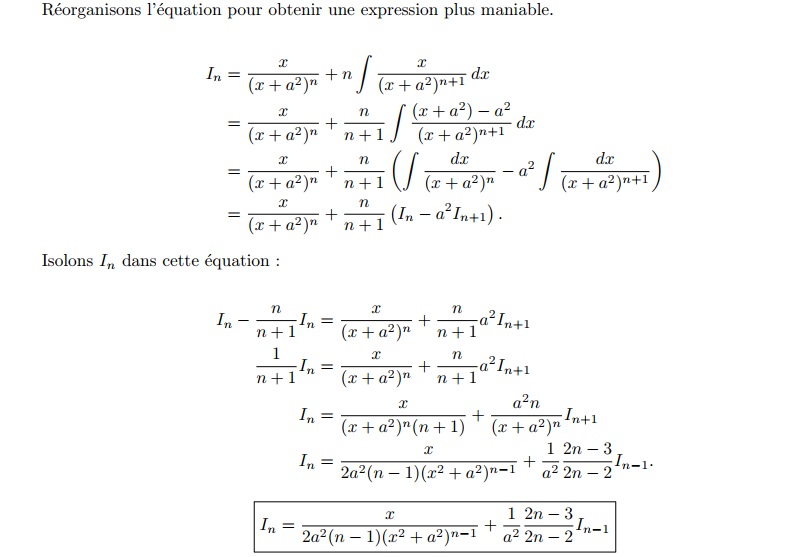
\includegraphics[width=0.6\textwidth]{images/calcul_integral/calcint-039-000.png}
\captionof{figure}{\small Régime transitoire RC : évolution de la tension $u_C(t)$ et du courant $i(t)$ lors de la charge et de la décharge.}
\end{center}
\begin{center}

\includegraphics[width=0.6\textwidth]{images/calcul_integral/calcint-039-001.png}
\captionof{figure}{\small Décroissance exponentielle de l'énergie $E(t)$ stockée dans le condensateur au cours de la décharge.}
\end{center}

\ifdefined\inMainDoc\else\end{document}\fi
